\documentclass[10pt,openright,twoside,french]{book}

\input philippe2013
\input philippe2013_cours
\input philippe2013_sections
\input philippe2013_chapitre

%film: bout de code à transformer en commande? piqué à JCC sur un post sur fr.comp.tex

\newlength{\epais}
\setlength{\epais}{12pt}
\newlength{\maigre}
\setlength{\maigre}{0.2pt}
\newlength{\normal}
\setlength{\normal}{\arrayrulewidth}
\newcolumntype{I}{!{\vrule width \epais}}
\newcolumntype{i}{!{\vrule width 10\maigre}}
\newcommand*\Hepais[1]{%
  \noalign{\global\setlength{\arrayrulewidth}{0.35\epais}}%
  \cline{#1}%
  \noalign{\global\setlength{\arrayrulewidth}{0.5\normal}}%
}
%\newcommand*\Hmaigre[1]{%
%  \noalign{\global\setlength{\arrayrulewidth}{\maigre}}%
%  \cline{#1}%
%  \noalign{\global\setlength{\arrayrulewidth}{\normal}}%
%}
\newcommand{\film}[6]{
\begin{tabular}{i*{18}{cI}}
  \Hepais{1-18}
        &&&&&&&&&&&&&&&&&\\
  \Hepais{1-18}
        \multicolumn{6}{ici}{} & \multicolumn{6}{c}{} & \multicolumn{6}{ici}{}\\

        \multicolumn{6}{ici}{\begin{minipage}[c]{{0.2\linewidth}}\centering{#1}\end{minipage}}
            &
        \multicolumn{6}{c}{\begin{minipage}[c]{{0.2\linewidth}}\centering{#2}\end{minipage}}
            &
        \multicolumn{6}{ici}{\begin{minipage}[c]{{0.2\linewidth}}\centering{#3}\end{minipage}}\\

        \multicolumn{6}{ici}{} & \multicolumn{6}{c}{} & \multicolumn{6}{ici}{}\\

    \Hepais{1-18}
        &&&&&&&&&&&&&&&&& \\
    \Hepais{1-18}
        \multicolumn{6}{c}{} & \multicolumn{6}{c}{} & \multicolumn{6}{c}{}\\

        \multicolumn{6}{c}{\begin{minipage}[t]{{0.2\linewidth}}#4\end{minipage}}
            &
        \multicolumn{6}{c}{\begin{minipage}[t]{{0.2\linewidth}}#5\end{minipage}}
            &
        \multicolumn{6}{c}{\begin{minipage}[t]{{0.2\linewidth}}#6\end{minipage}}
\end{tabular}
}



\setcounter{chapter}{12}
\begin{document}

\renewcommand\PartProgramme{Géométrie}
\chapter{Vecteurs}\label{ch_vecteurs}

\section{Vecteur et représentants}

\subsection{Translation}

\begin{Defi}\label{Defi_Translation}
    Soit $A$ et $B$ deux points donnés.\par
    La \ipt{translation} qui transforme le point $A$ en $B$ est la transformation géométrique qui, à tout point $M$, associe l'unique point $N$ tel que les segments $[AN]$ et $[BM]$ ont le même milieu ; autrement dit, tel que le quadrilatère $ABNM$ est un parallélogramme \textbf{(attention à l'ordre des lettres !)}.
    \begin{center}
        \begin{tikzpicture}[scale=0.75,>=latex]
            \tkzDefPoint(5,0){A}
            \draw (A) node[right] {\footnotesize $A$};
            \tkzDefPoint(2,1){B}
            \draw (B) node[left] {\footnotesize $B$};
            \tkzDefPoint(4,2){M}
            \draw (M) node[right] {\footnotesize $M$};
            \tkzDefPoint(1,3){N}
            \draw (N) node[left] {\footnotesize $N$};
            \draw (A)--(B)--(N)--(M)--cycle;
            \draw[dashed] (M)--(B);
            \draw[dashed] (A)--(N);
            \tkzInterLL(A,N)(B,M)\tkzGetPoint{K}
            \tkzMarkSegments[mark=s|](N,K K,A)
            \tkzMarkSegments[mark=s||](M,K K,B)
            \draw[line width=0.75pt,->,color=red] (A) -- (B);
        \end{tikzpicture}
    \end{center}
\end{Defi}

\begin{Rmq}
    Lorsque les points $A$, $B$ et $M$ sont alignés, le quadrilatère $ABNM$ obtenu est un parallélogramme plat.\par
    Les segments $[AN]$ et $[BM]$ ont toujours le même milieu.
\end{Rmq}

\begin{Defi}
    La transformation qui transforme $A$ en $B$ est appelée translation de \ipt{vecteur} $\vect{AB}$.\par
    On la note souvent $t_{\vect{AB}}$.
\end{Defi}

\subsection{Représentant d'un vecteur}

\begin{Defi}
    D'après la définition \ref{Defi_Translation}, $t_{\vect{AB}} = t_{\vect{MN}}$ donc on dira que les vecteurs $\vect{AB}$ et $\vect{MN}$ sont égaux.\par
    Le vecteur $\vect{AB}$ possède trois caractéristiques :
    \begin{description}
        \item[sa \ipt{direction} :] correspond à la direction de la droite $(AB)$ ; autrement dit, la direction représente l'\textit{inclinaison} du vecteur ;
        \item[son \ipt{sens} :] correspond au sens de \textit{déplacement} de $A$ vers $B$ donné par la translation qui transforme $A$ en $B$. Sur un dessin, on l'indique par une flèche.
        \item[sa \ipt{norme} :] correspond à la longueur du segment $[AB]$, notée $AB$ ou bien $\norme{\vect{AB}}$.
    \end{description}
\end{Defi}

\begin{Exemple}
    Les vecteurs $\vect{AB}$ et $\vect{BA}$ ont la même direction et la même norme. En revanche, ils sont de sens contraire. Ils ne sont donc pas égaux. On dit qu'ils sont \iptb{opposés}.
\end{Exemple}

\begin{Defi}
    Deux vecteurs qui ont la même direction sont appelés des vecteurs \ipt{colinéaires}.
    \begin{center}
        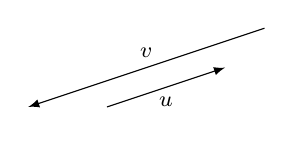
\begin{tikzpicture}[scale=0.5,>=latex]
            \draw[->] (0,0) -- ++(3,1) node[midway,below] {\footnotesize$\vect u$};
            \draw[<-] (-2,0) -- ++(6,2) node[midway,above] {\footnotesize$\vect v$};
        \end{tikzpicture}
    \end{center}
\end{Defi}

\subsection{\'Egalité de vecteurs}
\begin{Prop}[(admise)]
    \begin{tabular}{r@{$\qLRq$}l}
        $\vect{AB}= \vect{MN}$ & $N$ est l'image de $M$ par la translation qui transforme $A$ en $B$ \\
                                               & $[AN]$ et $[BM]$ ont le même milieu \\
                                               & $ABNM$ est un parallélogramme \\
                                               & $\vect{AB}$ et $\vect{MN}$ ont le même sens, la même direction et la même norme.
    \end{tabular}
\end{Prop}

\begin{Defi}
    Les vecteurs qui ont les mêmes caractéristiques que le vecteur $\vect{AB}$ sont appelés des \ipt{représentants} du vecteur $\vect{AB}$. Il en existe une infinité.
\end{Defi}

\section{Somme de vecteurs}

\begin{Defi}
    Soient $A$, $B$ et $C$ trois points.\par
    La \iptb{somme}\index{vecteur!somme} de deux vecteurs $\vect{AB}$ et $\vect{BC}$ est le vecteur associé à la translation obtenue en appliquant successivement $t_{\vect{AB}}$ et $t_{\vect{BC}}$.\par
    On écrit alors la \ipt{relation de Chasles} : $\vect{AB} + \vect{BC} = \vect{AC}$.
    \begin{center}
        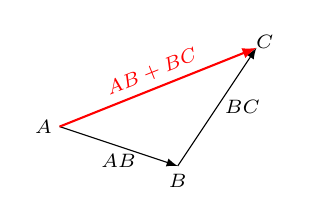
\begin{tikzpicture}[scale=0.5,>=latex]
        \scriptsize
            \draw[->] (0,0) node[left] {$A$} -- (3,-1) node[below] {$B$} node[midway,below] {$\vect{AB}$};
            \draw[->] (3,-1) -- (5,2) node[above right=-3pt] {$C$} node[midway,right] {$\vect{BC}$};
            \draw[->,red,line width=0.75pt] (0,0) -- (5,2) node[midway,above,sloped] {$\vect{AB}+\vect{BC}$};
        \end{tikzpicture}
    \end{center}
\end{Defi}

\begin{center}
    \small
        \film%
            {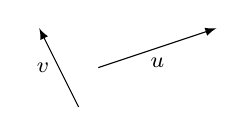
\begin{tikzpicture}[scale=0.5,>=latex]
                \draw[->] (0,0) -- ++(3,1) node[midway,below] {\footnotesize$\vect u$};
                \draw[->] (-0.5,-1) -- ++(-1,2) node[midway,left] {\footnotesize$\vect v$};
            \end{tikzpicture}}%
            {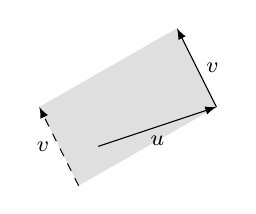
\begin{tikzpicture}[scale=0.5,>=latex]
                \fill[color=lightgray!50] (-0.5,-1) -- (3,1) -- (2,3) -- (-1.5,1) -- cycle;
                \draw[->] (0,0) -- ++(3,1) node[midway,below] {\footnotesize$\vect u$};
                \draw[->,dashed] (-0.5,-1) -- ++(-1,2) node[midway,left] {\footnotesize$\vect v$};
                \draw[->] (3,1) -- ++(-1,2) node[midway,right] {\footnotesize$\vect v$};
            \end{tikzpicture}}%
            {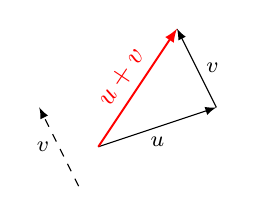
\begin{tikzpicture}[scale=0.5,>=latex]
                \draw[->] (0,0) -- ++(3,1) node[midway,below] {\footnotesize$\vect u$};
                \draw[->,dashed] (-0.5,-1) -- ++(-1,2) node[midway,left] {\footnotesize$\vect v$};
                \draw[->] (3,1) -- ++(-1,2) node[midway,right] {\footnotesize$\vect v$};
                \draw[->,red,line width=0.7pt] (0,0) -- ++(2,3) node[midway,above,sloped] {$\vect{u}+\vect{v}$};
            \end{tikzpicture}}%
            {\textbf{\'Etape 1 :} On veut représenter $\vect u + \vect v$.}%
            {\textbf{\'Etape 2 :} On dessine un représentant de $\vect v$ à l'extrémité de $\vect u$.}%
            {\textbf{\'Etape 3 :} On utilise la relation de Chasles.}
\end{center}

\begin{Prop}[(en utilisant la relation de Chasles)]
\begin{minipage}{0.7\linewidth}
    On souhaite ajouter deux vecteurs de même origine.\par
    $\vect{AB} + \vect{AC} = \vect{AD}$ tel que $ABDC$ est un parallélogramme.
\end{minipage}
\begin{minipage}{0.25\linewidth}
    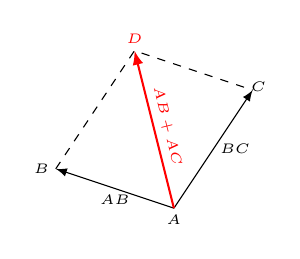
\begin{tikzpicture}[scale=0.5,>=latex]
        \tiny
            \draw[<-] (0,0) node[left] {$B$} -- (3,-1) node[below] {$A$} node[midway,below] {$\vect{AB}$};
            \draw[->] (3,-1) -- (5,2) node[above right=-3pt] {$C$} node[midway,right] {$\vect{BC}$};
            \draw[->,red,line width=0.75pt] (3,-1) -- ++(-1,4) node[midway,above,sloped] {$\vect{AB}+\vect{AC}$} node[above] {$D$};
            \draw[dashed] (0,0)--(2,3)--(5,2);
    \end{tikzpicture}
\end{minipage}
\end{Prop}

\section{Coordonnées dans un repère}

\begin{Defi}
    Les \iptb{coordonnées d'un vecteur}\index{vecteurs!coordonnées} $\vect u$ dans un repère \OIJ sont les coordonnées de l'unique point $M$ tel que $\vect{OM} = \vect u$.
\end{Defi}

\begin{Prop}
    Dans un repère, on considère deux points $A(x_A \pv y_A)$ et $B(x_B \pv y_B)$. Alors le vecteur $\vect{AB}$ a pour coordonnées $x_{\vect{AB}}$ et $y_{\vect{AB}}$ tels que :
    \[x_{\vect{AB}} = x_B - x_A \qetq y_{\vect{AB}} = y_B - y_A.\]
\end{Prop}

\begin{Rmq}
    Les coordonnées du vecteur $\vect{AB}$ correspond aux déplacements horizontal et vertical pour se rendre de $A$ vers $B$.
\end{Rmq}

\begin{center}
    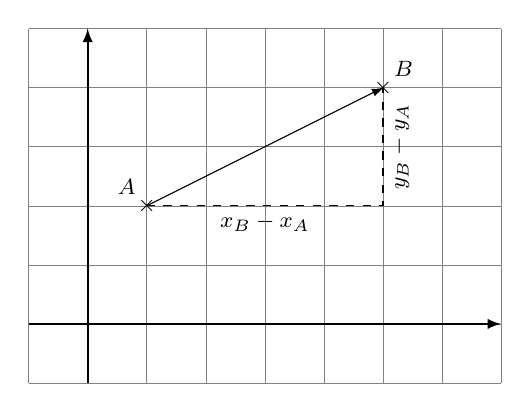
\begin{tikzpicture}[scale=0.75,>=latex]
    \footnotesize
        \draw[help lines] (-1,-1) grid (7,5);
        \draw[->, line width = 0.7pt] (-1,0)--(7,0);
        \draw[->, line width = 0.7pt] (0,-1)--(0,5);
        \draw[->] (1,2) node {$\times$} node[above left=1pt] {$A$} -- (5,4) node {$\times$} node[above right=1pt] {$B$};
        \draw[dashed,line width=0.5pt] (1,2) -- (5,2) node[below,midway] {$x_B-x_A$} -- (5,4) node[below,sloped,midway] {$y_B-y_A$};
    \end{tikzpicture}
    
    Ici, $A(1\pv2)$ et $B(5 \pv 4)$ donc $\vect{AB} \binom 42$.
\end{center}

\begin{Prop}
    Soient $\vect u\binom{x_{\vect{u}}}{y_{\vect{u}}}$ et $\vect v\binom{x_{\vect{v}}}{y_{\vect{v}}}$ deux vecteurs dans un repère. Alors :
    \[\vect u + \vect v\binom{x_{\vect{u}}+x_{\vect{v}}}{y_{\vect{u}}+y_{\vect{v}}} \qetq k\vect u\binom{kx_{\vect{u}}}{ky_{\vect{u}}}.\]
\end{Prop}

\begin{Prop}
    \begin{tabular}{r@{$\quad\Leftrightarrow \quad$}l}
        $\vect u$ et $\vect{v}$ sont colinéraires & il existe $k \in \R$ tel que $\vect v = k\vect u$\\
                                                                      & $x_{\vect u} \times y_{\vect v} - y_{\vect u} \times x_{\vect v} = 0$.
    \end{tabular}
\end{Prop}

\begin{Exemple}
    $A(1 \pv 1)$ \quad $B(4\pv 2)$\quad $C(4 \pv 1)$ \quad $D(10\pv 3)$. Les droites $(AB)$ et $(CD)$ sont-elles parallèles ?\par\medskip
    On a $\vect{AB}\binom 3 1$ et $\vect{CD}\binom 6 2$.\par\medskip
     $3 \times 2 - 1 \times 6 = 0$ donc les vecteurs $\vect{AB}$ et $\vect{CD}$ sont colinéaires donc les droites $(AB)$ et $(CD)$ sont parallèles.\par\medskip
    On remarque que $\vect{CD}= 2\vect{AB}$.
\end{Exemple}

\end{document}
